\documentclass{article}
\setlength{\headheight}{13.59999pt}
\usepackage[utf8]{inputenc}

\title{Luminosity function}
\author{Henrik Andrews}

\usepackage{natbib}

\usepackage{subcaption}
\usepackage[ portrait, margin=2cm]{geometry}
\usepackage{graphicx}
\usepackage{amsmath}
\usepackage{upgreek}
\usepackage{bbold}
\usepackage{fancyhdr}
\usepackage{mathtools}
\usepackage{tabularx}
\usepackage{lipsum}
\usepackage{pdfpages}
\setlength{\parindent}{0em}
\setlength{\parskip}{1em}
\usepackage{caption}
\usepackage{multicol}

\usepackage{float}
\newcommand{\HRule}[1]{\rule{\linewidth}{#1}}
\usepackage{listings}
\usepackage{color} %red, green, blue, yellow, cyan, magenta, black, white
\definecolor{mygreen}{RGB}{28,172,0} % color values Red, Green, Blue
\definecolor{mylilas}{RGB}{170,55,241}
\definecolor{backcolour}{rgb}{0.95,0.95,0.92}
\begin{document}

% title source: https://www.overleaf.com/project/6021d9e4632b9ef90aa8d238
\title{ \normalsize \textsc{AREA}
	\\ [2.0cm]
	\HRule{0.5pt} \\
	\LARGE \textbf{\uppercase{Theme}}		
	\\ Title\\
	\HRule{2pt} \\ [0.5cm]		
%fix the university logo !!!!!!!!!!!!!!!!!!!!!!!!
	\vspace{6cm}
	\begin{figure}[htp]
    \centering
    
\includegraphics[width=.2\textwidth]{Logo-Ntnu.svg.png}
    \end{figure}
	}

\author{
    \normalsize 
	\textbf{Henrik Døvle Andrews } \\
	Norwegian university of Science and Technology \\ 
}

\maketitle
\setcounter{page}{ 0 }

\newpage

\pagestyle{fancy}
\fancyhf{}
\setlength\headheight{12pt}
\fancyhead[L]{Henrik Døvle Andrews}
\fancyhead[R]{Luminosity functions}
\fancyfoot[R]{Page \thepage \:}
\setcounter{page}{1}


\maketitle

% Abstract
\begin{abstract}
\lipsum[1] % Replace with your abstract text
\end{abstract}

\newpage 
% Summary (you might use a simple section for this)
\section*{Summary}
\lipsum[2] % Replace with your summary text

\newpage
% Acknowledgments
\section*{Acknowledgments}
\lipsum[3] % Replace with your acknowledgment text

\newpage
% Table of Contents (optional)
\tableofcontents

\newpage
% List of Figures
\listoffigures

% List of Tables
\listoftables

-abstract 
-sammendrag
-acknowledgments
-list of figure
-list of tables

\newpage

\section{Introduction}

\section{The ever expanding universe}
In order to investigate sources very far away from an observer it is important to understand the influence this distance 
has on your desired observablea. Therefore in astrophysics and astronomy in general there are distances created to take into account the effects of an expanding universe. 


\subsection{Comsographic parameters}

The most notorious parameter due to its controversy when first discovered is the Hubble constant $H_0$. 
This parameter sets the recession speed of a point at proper distance $d$ and our current position via this simple relation. $v = H_0 d$ 
The subscript $0$ refers to the present epoch signifiing that $H_0$ is not static butchanges with time. 
The precise value of $H_0$ is quite debated so its commenly expressed in a parameterized form. 
$$
H_0= 100\frac{km}{s}\frac{1}{Mpc} h 
$$
where $h$ is a dimensionless number that according to current knowledge  can take the value between $0.5$ to $0.8$ reflecting the range of answers collected from recent work. 

Beyond its basic definition,$H_0$ also allows for the derivation of two significant cosmic scales:

\textbf{Hubble Time ($t_H$) }: Defined as the inverse of 
$H_0$ , $t_H$ provides an estimate of the age of the universe. 
It sets a scale for the time since the Big Bang, assuming the universe has been expanding at a constant rate. The equation 
$t_H = \frac{1}{H_0} \approx 14 \quad \text{Billon years}$ offers a simple way to approximate this expansive timescale.


\textbf{Hubble Distance ($D_H$) }: This is a measure of the distance over which the universe's expansion is significant. Calculated as 
$D_H = \frac{c}{H_0} \approx 4.4 \quad \text{Gly}$, where $c$ is the speed of light, 
it represents a critical boundary in observational cosmology. %Beyond this distance, the expansion of the universe dominates the motion of galaxies, providing a fundamental constraint for cosmological observations and theories.

\subsection{Shape of the universe}


The shape and expansion of the universe are central themes in cosmology, but in order to do that one needs to define the structure of the universe and its contents. 
In this paper and in many articles the universe is
often explored through the lens of the flat Lambda Cold Dark Matter ($\Lambda$CDM) model. 
This model, widely accepted in contemporary cosmology, provides a framework for understanding the universe's composition and its expansion dynamics by assuming as the name suggests no curvature.
In the $\Lambda$CDM model, two key parameters are important: the mass density of the universe, $\rho_0$, and the cosmological constant, $\Lambda$.
These parameters, which evolve over time, are a part in defining the metric tensor in general relativity, thereby allowing us to model the curvature of the universe based on its initial conditions.
These parameters are often expressed as dimensionless variables:

$$
\Omega_m = \frac{8\pi G\rho_0}{3H_0^2}
$$

$$
\Omega_\Lambda = \frac{\Lambda c^2}{3H_0^2}
$$

Here, $\Omega_m$ represents the matter density parameter, encompassing both ordinary (baryonic) matter and dark matter. 
$\Omega_\Lambda$, on the other hand, corresponds to the density parameter associated with the cosmological constant, which is often interpreted as dark energy.




In general one has a third density parameter $\Omega_k$ which defines the curvature of spacetime and the relationship between these paramters is expressed as: 

$$
\Omega_m + \Omega_\Lambda + \Omega_k = 1
$$


In a flat universe one has $\Omega_k = 0$ and the universe is dominated by dark energy and dark matter. The model used in this paper and the papers cited if not expressed otherwise is the flat $\Lambda$CDM model where the parameters take the values of 
$\Omega_\Lambda = 0.7$ and $\Omega_m = 0.3$. These values align with current obersvational data (refff).



\subsection{Redshift}
Redshift is defined as the fractional Doppler shift of emitting light. The Doppler effect is a known effect on different observables in our universe where the relative motion of sources to observers will impact the observable. The redshift is quantified for a light source as 

\begin{equation}
    z = \frac{\nu_e}{\nu_o}-1 = \frac{\lambda_o}{\lambda_e}-1
\end{equation}

Here $o$ refers to the observed quantity and $e$ the emmited. Due to the expansion of the universe the light emitted from a distant source will be increasingly redshifted the further away it is.
In these scenarios the redhsift serves as a distance measure, allowing  us to deduce distances to faraway objects.



\subsection{Comoving distance}
\label{sec:comoving_distance}


Comoving distance is an important concept in cosmography, 
acting as a standard unit for various distance measurements in the universe. 
This distance, often termed the line-of-sight distance for an observer on Earth, 
remains constant even as objects expand with the Hubble flow. 
To calculate the total comoving distance ($D_c$) to an object, 
one integrates the differnetial comoving distances ($\delta D_c$) along the line of sight, starting from redshift 
$z=0$ to the object. This integration necessitates consideration of the universe's parametric composition and the $\delta D_c$ is expressed as

\begin{equation}
    \delta D_c = \frac{D_H}{E(z)}dz
\end{equation}
where the function $E(z)$ is defined as
\begin{equation}
    E(z)  = \sqrt{\Omega_m(z+1)^3 +\Omega_k (1+z)^2 + \Omega_\Lambda  }
\end{equation}
Here, 
$E(z)$ incorporates the density parameters previously discussed and the redshift 
$z$. It also relates to the Hubble constant observed by hypothetical observer at redshift $z$, expressed as 
$H(z) = H_0 E(z)$.

One then recives the comoving distance $D_c$ from 
\begin{equation}
    D_c =D_H \int_0^z\frac{dz}{E(z)}
\end{equation}

In addition to the line of sight one needs to define the transverse comoving distance $D_m$. This distance 
relates two points in the nights sky at the same redshift seperated by an angle $d\theta$. The actual distance
between them $d\theta D_m$ will then vary depending on the curvature of the universe. This reltionship is summariesed in the followin equation
which accounts for differen geometries.

$$
D_m =
\begin{cases}
  D_h\frac{1}{\sqrt{\Omega_k}}sinh(\frac{\sqrt{\Omega_k}D_c}{D_H}) & \text{if } \Omega_k > 0 \\
  D_c& \text{if } \Omega_k = 0 \\
  D_h\frac{1}{\sqrt{|\Omega_k|}}sin(\frac{\sqrt{|\Omega_k|}D_c}{D_H}) & \text{if } \Omega_k < 0
\end{cases}
$$

The different cases corresponds to hyperbolic, flat and spherical geometry respectively. The true nature 
of the universe is still unknown but the recent observations indicate a flat universe. grand design!!!








\subsection{Luminosity distance}
The luminosity distance $D_l$ is defined through the relation between 
the bolometrix flux $F$ of a source and its bolometric luminosity $L$. bolometric flux is the energy received per unit time per unit area, while bolometric luminosity is the total energy emmited per unit time.
The luminosity distance is defined as
\begin{equation}
    D_l = \sqrt{\frac{L}{4\pi F}}
\end{equation}

This fomula essentially describes the loss of energy due to the expansion of the universe. It reflects how the observed flux at the observer's location differs based on the distance from the source and the intrinsic luminosity emmited. 

It is related to the transverse comoving distance via 

\begin{equation}
    D_l = (1+z)D_m
\end{equation}

This of course is for bolometric quantities, but if one wants to calculate the spectral 
flux/ differential flux one need to take into account a correction. This correction comes 
from the fact that one is viewing a redshifted object. The object is emmiting in a different band than 
observed. The spectrum of the differnetial flux $F_\nu$ is related to the spectral luminosity via
\begin{equation}
    F_\nu = (1+z) \frac{L_{(1+z)\nu}}{L_\nu}\frac{L_\nu}{4\pi D_l^2}
\end{equation}


All these equations listed help include the effects of an expanding universe when astronomers study distant objects and their properties. 

\section{High energy particles}
In this section i will discuss the different types of high energy particles that are of interest in this paper, i.e neutrinos and ultra high energy cosmic rays(UHECRs).
I will breifly discuss their generation and how they are detected. Then introduce how they lose energy in their journey to earth, and lastly calculate the emmisivity of their hypothetical sources from ground 
observations here on earth. 

\subsection{Acceleration of high energy particles}

In order to reach high energy, particles need to be accelrated. 
Knowing the exact source of acceleration can be difficult since we do not know the sources, but nontheless one can put constraints on any source due to some simple arguments.
By arguing that the acceleration needs to be of a certain strength and that the particle being accelerated need to stay confined witihn the accelerator for long enough one can put constraints on the source.
This is called the Hillas criterion and is a simple way of estimating the maximum energy a particle can reach in a given source.(ref hillas)

For relativistic particle with charge $Z$ and energy $\epsilon$ in a magnetic field of strength $B$ one can define the larmor radius


\begin{equation}
    R_L = \frac{\epsilon}{ZB}
\end{equation}

By arguing that the definition of confinment of a particle to a source is by equtating the larmor radius to the size of the source one can 
easily derive the maximum acheivable energy for a particle as follows. (ref M. Bustamante. https://cds.cern.ch/record/1249755/files/p533.pdf)

\begin{equation}
    \epsilon_{max} = ZBR
\end{equation}

Via this method one can illustra the potential candidates needed to produce the required and importantly observed high energy particles. 
This requirement is named the hillas criterion after G. Hillas who first proposed this method.
In figure \ref{fig:hillas_c} one can see the different candidates for the acceleration of two different ions, protons and iron. One of the candidates is the AGN, which is the focus of this paper.

\begin{figure}
    \centering
    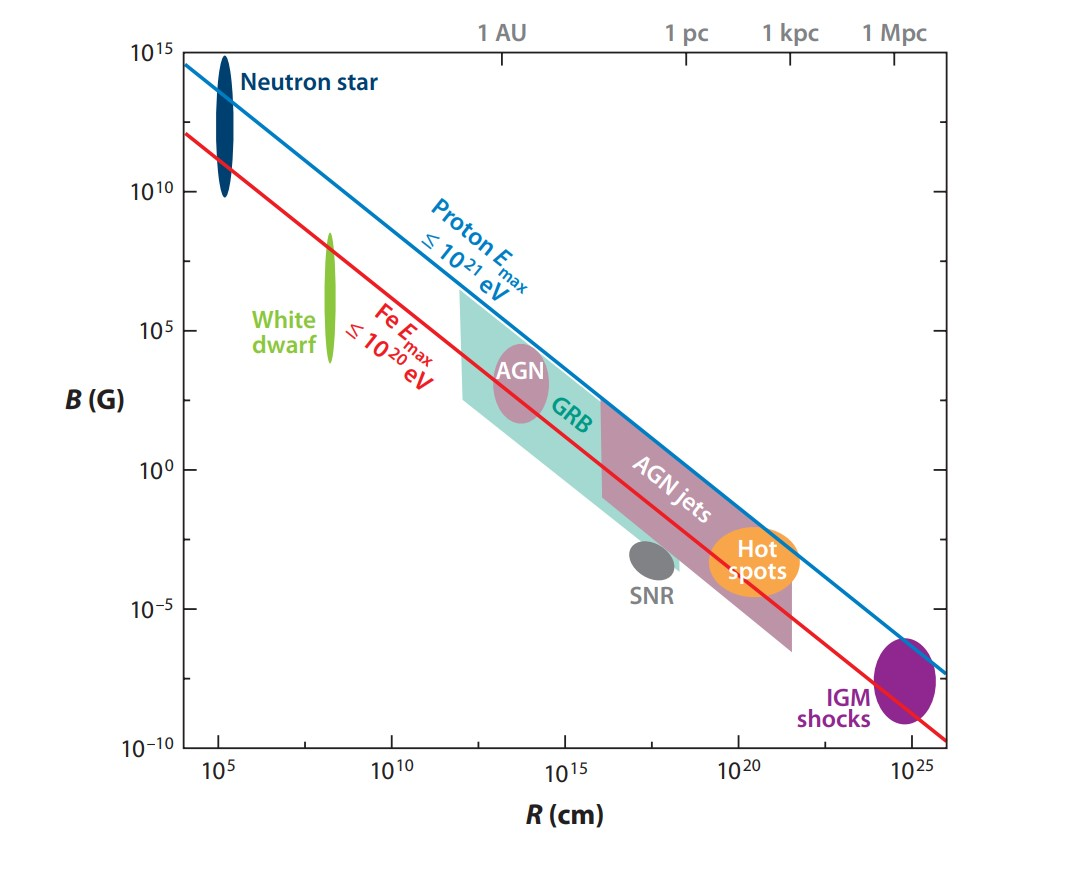
\includegraphics[width = 0.5\textwidth]{hillas_criterion.jpeg}
    \caption{Hillas criterion for proton (blue line) and iron (red line) accelerated up to $10^{20}eV$ and $10^{21}eV$ respectively. Image taken from \cite{doi:10.1146/annurev-astro-081710-102620}}
    \label{fig:hillas_c}
\end{figure}


One can try to build sources in bottom up models, and then it is necessaery to understand the different processes that can accelerate particles to high energies, here i will breifly go through some. 

\textbf{One-shot acceleration}:
In the precence of an ordered field one can accelerate particles in an continous manner. This could be the feature of some astrophysical objects such as neutron stars and black holes. (ref cern paper)


\textbf{Diffusive acceleration/ Fermi acceleration}
In regions where one has high varaibility in the magnetic field strength one can accelerate particles in burst. 
This is called diffusive acceleration and the most common way of this happening is through first and second order fermi acceleration.
The second order fermi acceleration is the simplest and is based on the fact that particles can gain energy by bouncing back and forth between magnetic clouds which acts as mirrors. 
This is a stochastic process and the average energy gain can be showed to be proportional $(\frac{v}{c})^2$. Here $v$ is the speed of the cloud 
and $c$ the speed of the particle. This is a slow process due to the scarcity of clouds and therefore it is not a prefered method.
The first order fermi acceleration happens when particles collide with strong shock fronts. These shock fronts can be quite a bit faster than our interstellar clouds
and when a particle moves through the shock it gains energy proportional to $\frac{v}{c}$. In addition to this there is a probability that the particle will stay in the accelerating region and 
experience several shocks accelerations. 

By knowing how particles can accelerate and their potential sources one can continue an look at the two particles of question in this paper. 
Neutrinos and UHECRs.
\subsection{UHECRs}

UHECRs are simply put charged particles that are bombarding earth with energy exceeding .... (1exaelectronvolt ($10^{18}$ eV)). The origin of 
these particles are still a mystery but  due to their high energies they are thought to be extragalactic in origin and due to the hillas criterion need to be suffciently good accelerators.
The composition of UHECRs are mostly protons and heavier nuclei such as helium or iron, and when these particles interact with the atmosphere they produce a shower of secondary particles.
The air showers could also give extra infromation such as direction, but due to the nature of UHECRs the location of their source is
difficult to pinpoint. This is due to the fact that UHECRs are charged particles and therefore are deflected by the magnetic fields it encounter.

\subsubsection{Production and Energy loss}
The neceassary requirements for a UHECRs is a charge particle and a powerfull accelerator. From the hillas criterion one can see that there are several candidates so i will assume that these reuirements are fufilled and we have a particle with sufficent energy that has been released from its source.
An equal interesting part is the journey of the particle to earth since during the acceleration and during the journey to earth the UHECRs will lose energy. The important parameters for this energy loss is its  composition  and its enviroment. In addition as mentioned before
, the intersteller magnetic field will also deflect the particles and therefore the direction of the particle will be changed. These effects are important parameters since it limits the 
distance a particle can travel before its start energy becomes unreasonable, and thefore limits the local volume in which it can be produced. 
Here i will briefly discuss the different energy loss mechanisms. 
\textbf{Photo-pair production}

\begin{equation}
    p + \gamma \rightarrow p + e^- + e^+
\end{equation}
For UHECRs the most potent sink of energy is the Bethe-Heitler process. In this process a proton of sufficent energy interacts with the 
the photon field in its vicinity and produces a pair of electron and positron. The photon field can vary from the cosmic microwave background to the generated field from different sources. 
The energy loss of this process is quite small $\sim \frac{2m_e}{m_p}= 10^{-3}$ of the original energy of the proton, but the process is very common and therefore it is a significant energy loss over time.


\textbf{Pion production thorugh delta resonance}
\begin{equation}
    p + \gamma \rightarrow \Delta^+ \rightarrow (p + \pi^0)\quad \text{or} \quad (\pi^+ + n)
    \label{eq:delta_resonance}
\end{equation}

Given enough energy the proton can interact with the photon field and produce a delta resonance. This resonance can then decay into a pion and a proton or a neutron and a pion. 
This process is important since it also puts an upper limit on the UHECRs energy for intergalactic particles. 
This limit, called the Greisen-Zatsepin-Kuzmin (GZK) limit comes from the UHECRs interacting with the cosmic microwave background in this delta resonance process. The limit caps proton energy at $5\times 10^{19}$ eV.

\textbf{photodisintegration}
mabye include this. 

\subsubsection{Detection}
When a cosmic ray hits the atmosphere it will interact with the air molecules and produce a cascade of particles and light that can more easily be detected than 
the original cosmic ray.In addition, since the UHECR flux at high energy is extremly low (<1 particle per $km^2$ per year for $E > 10^{19}$ ) one need a large area to collect enough data. 
The best detectors to do this kind of work are the Pierre Auger observatory and the Telescope Array. 

The Pierre Auger observatory is located in Argentina and is the largest detector of its kind. It consists of 1660  Cherenkov detectors spread over 3000 km$^2$ and 27 fluorescence telescopes in four locations. With 
these instruments the observatory is very capable of reconstructing the air showers and therefore the original cosmic ray. The observatory has a blind spot in the night sky 
and therefore the observatory is complemented by the Telescope Array located in Utah. The Telescope Array is a smaller observatory with 507 scintillator detectors and 3 fluorescence telescopes. Combined they have been able to map the full sky of UHECRs.  

\subsubsection{Emissivity estimates}
\label{sec:emmisivity}

Now that one somwhat understand the nature of UHECRs one can try to make tangible estimates of the UHECRs sources. One such
estiamte is the emissivity of UHECR sources. An emmisivty is a measure of the energy released per unit time per unit volume. The question 
we can ask ourself is what is the neceassary emmisivity of UHECRs to explain the observed flux here on earth.


\begin{figure}
    \centering
    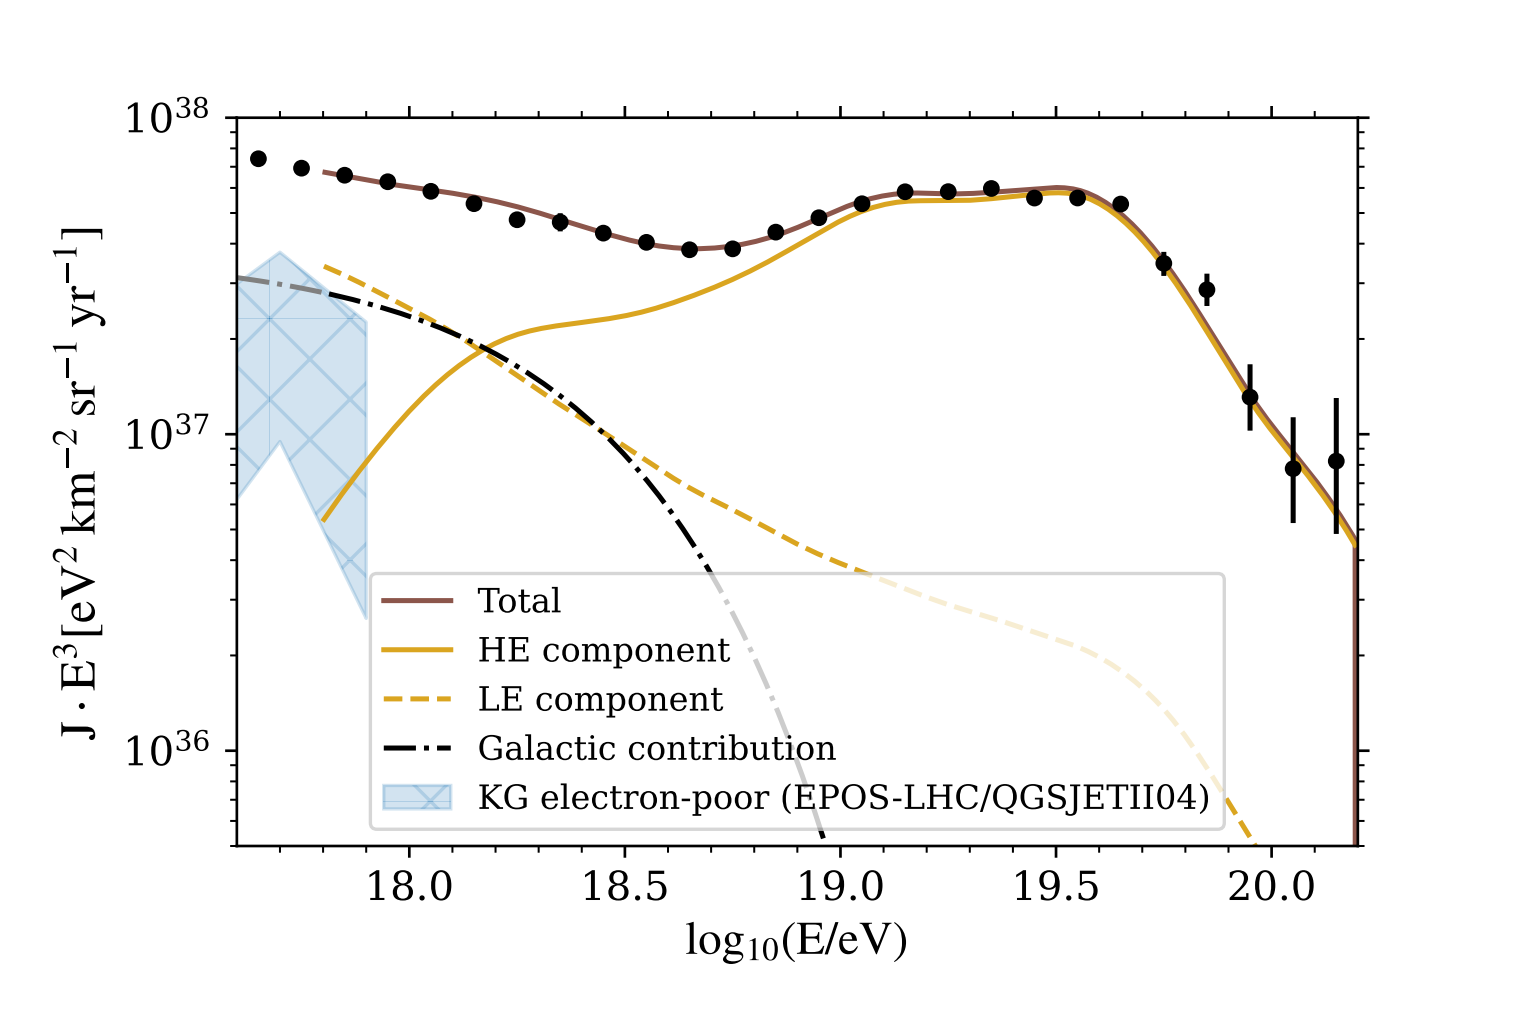
\includegraphics[width = 0.7\textwidth]{UHECRs.png}
    \caption{The diffuse flux of UHECRs as measured by the Pierre Auger observatory and the Telescope Array. The flux is seperated into galactic and extra galactic sources where the total spectrum follows the black dots. Image taken from \cite{Abdul_Halim_2023}}
    \label{fig:flux_UHECRs}
\end{figure}

Via observations from the Pierre Auger observatory and the Telescope Array one can observe and model the diffuse flux of UHECRs. The result is an isotropic flux and is represented in figure \ref{fig:flux_UHECRs} .  By seperating the 
flux into contribution from extra galactic sources and galactic sources one can estimate the reuqired energy density in the univers of extragalactic UHECRs. From here can define a the loss time for a UHECRs as the loss length divided by the speed of light $c$. This factor is depended on the differen method of energy loss for an UHECR. and 
then the emmsiivity of UHECRs produced by our sources as the energy density divided by the loss time.

To estimate a simple emmisivity for UHECRs one can use the following equation.

\begin{equation}
    \epsilon_{UHECR} = \frac{u_{UHECR}}{t_{loss}} = \frac{u_{UHECR}}{D_{loss}/c} = \frac{4\pi c \int_{E_0}^{E_{max}}J_{extragalactic}(E)E dE}{c D_{loss}} \approx 7\times 10^{44} \frac{erg}{Mpc^3 yr}
\end{equation}

Here $u_{UHECR}$ is the energy density of UHECRs, $t_{loss}$ is the loss time, $D_{loss}$ is the loss distance, $J(E)$ is the flux of UHECRs, $E_0$ is the minimum energy of the flux where it is dominated by extragalactic UHECRs, and $E_{max}$ is the maximum energy of extragalactic UHECRs.
The value of $\epsilon_{UHECR}$ is caulcated in the script avaible on github by using data from  Auger \cite{thepierreaugercollaboration2017pierre}


\subsection{Neutrinos}

The second particle of interest is the neutrino. Neutrinos compared to UHECRs are neutral particles that are produces in various processes in the universe.
The most common and well know is the fusion reaction in the sun where neutrinos are produced in the pp chain. On the other hand the neutrinos of focus in this paper 
are high energy neutrinos that are likley produced in the same sources as our UHECRs.



\subsubsection{Production and Energy loss}
The production of the highest energy neutrinos are thought to be produced in the same sources as UHECRs 
and i will go through the most probable way of producing high energy neutrinos in sources such as AGNs.

\textbf{Hardonic processes}
Hardonic procesess have the ability to release neutrinoes with a suffuciently high energy to explain the obersvations here on earth. 
Processes such as nuclear interactions are limitied by the bindign energy of the nucleaous and accelerating a neutrino after its production is difficult.
therefore a common way of producing the observed neutrinos is thorugh the decay of pions. The most important decay is the decay of charged pions into muons and muon neutrinos as seen in \ref{eq:pion_decay}


\begin{equation}
    \pi^+ \rightarrow \mu^+ + \nu_\mu \rightarrow e^+ + \nu_e + \nu_\mu + \bar{\nu_\mu}
    \label{eq:pion_decay}
\end{equation}

I will disucss two possible ways of producing these pion in two different enviroments. 


In proton rich enviroment where the protons are able to accelerate up to high energies one can produce pions through the following process
\begin{equation}
    p + p \rightarrow \begin{cases}
        \pi^+ + n+ p \\
        \pi^- + \pi^+ +p + p  \\
        \pi^0 + p+p
    \end{cases}
\end{equation}

The energy of these protons at a few GeV is enough to introduce the delta-baryon resonance and therefore it becomes more complicated.
The most efficient way of producing pions is through the already seen delta resonance when a proton interacts with a photon \ref{eq:delta_resonance}.
This process being similar to the cooling of UHECRs is a strong indicator that these two particles are produced in the same sources. 
After having produced our neutrinos it also becomes important to understand their behaviour during their travel to earth. Here I will higlight two points


\textbf{Neutrino oscillations}
In the previous paragraph I disussed the production of these neutrinos, but not their inital flavour.
The pion decay model is know to prodcue a flavour composition of $\nu_e : \nu_\mu : \nu_\tau = 1:2:0$. 
A naive thought would be an indentical composition observed on earth, but sadly this is not the case. 
The reason for this is that the neutrinos mass state has the ability to oscillate between the different flavours. Therefore the neutrinoes produced in the source will oscillate during their travel to earth and when they reach us one would expect a 
uniform mix of the three flavours, $\nu_e : \nu_\mu : \nu_\tau = 1:1:1$.

\textbf{Energy loss}
To model the travel of a neutrino of any flavour one only need to take into account the interaction of our neutrino with the expanding universe. Since it is so weakly interacting the only 
source of energy loss our flux of neutrinos will experience is the redshift created by the expansion of the universe. This redshift is the same as the one discussed in the previous section and our neutrinos 
behave the same way light does in this manner with a drop in energy proportional to $(1+z)$.



 

\subsubsection{Detection}
\begin{figure}
    \centering
    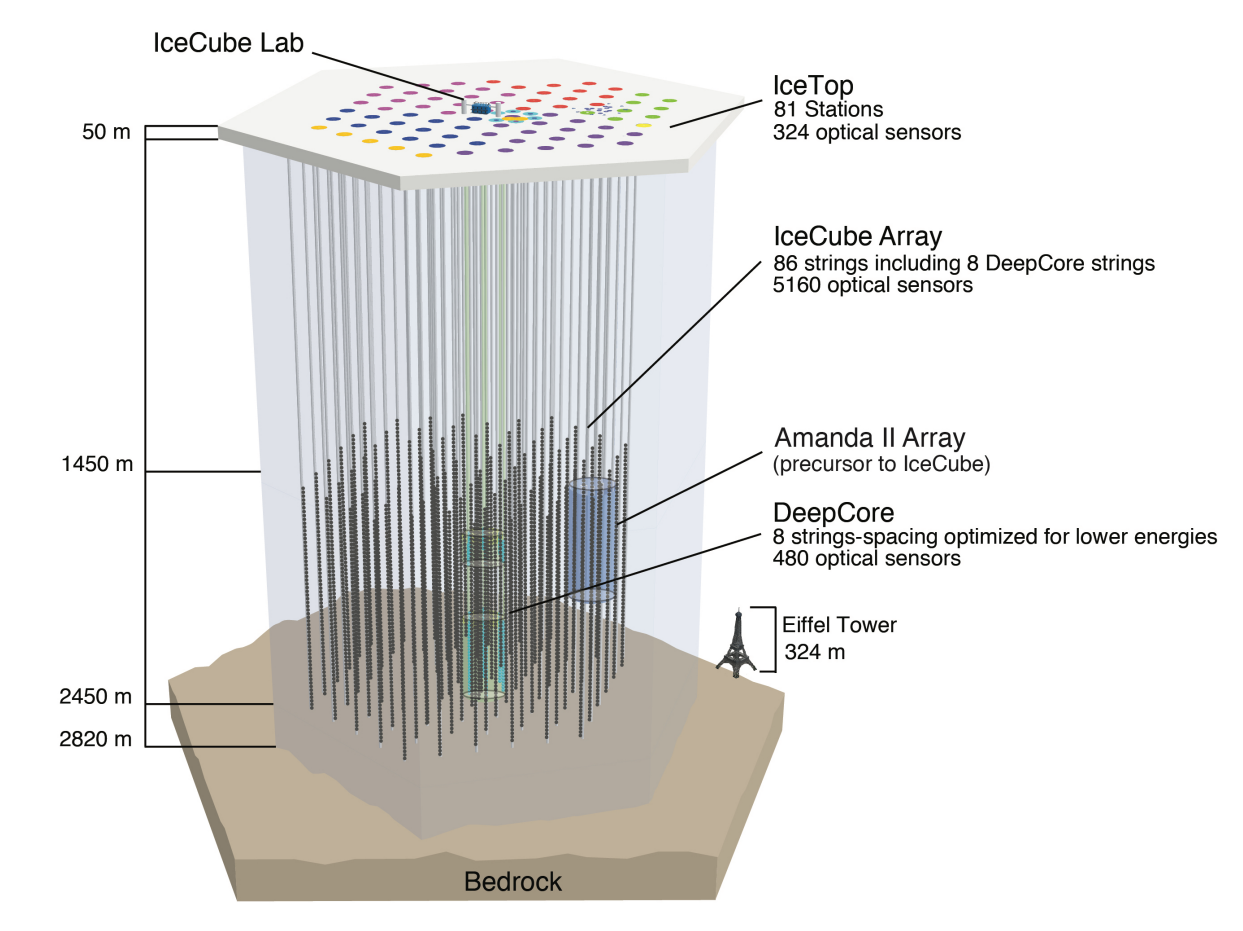
\includegraphics[width = 0.5\textwidth]{Ice_cube_layot.png}
    \caption{The ICE CUBE neutrino observatory. The detector is located at the south pole and is a large block of ice instrumented with photomultiplier tubes. Image taken from \cite{Andeen_2019}}
    \label{fig:Ice_cube}
\end{figure}

Neutrinos are weakly interacting matter particles and therefore are very difficult to detect. This makes them excellent candidates for the study of the universe since they can travel large distances without interacing, but make them 
quite difficult to detect with high accuracy. The most famous detector and the one used in this paper is the ICE CUBE neutrino observatory. This detector is precisely what it sounds. It is a large block of ice located at the south pole.
The observaotry uses the ice located deep in the south pole as a giant cherecencov detector. The ice is instrumented with photomultiplier tubes that can detect the Cherenkov radiation produced by neutrinos interacting with the ice. 
More precisely the observatory is fitted with 5160 photomultiplier tubes located at a depth of 1450-2450 m. The photomultipliers are divided into 86 strings of 60 modules each. The detector is also complemented by the DeepCore detector which is a denser array of photomultiplier tubes located in the center of the detector. See figure \ref{fig:Ice_cube} for a visual representation of the detector.
The energy range for this detector is from 10 GeV to 10 EeV. The interaction of neutrinoes with the water molcules in the ice can produce charged leptons( muons ,electrons or taus). These charged particles if energetic enough will then produce Cherenkov radiation which can be detected by the photomultiplier tubes.


\subsubsection{Emissivity estimates}
\label{sec:emmisivity_neutrinos}

Armed with the required knowledge above one can also make simple arguments for the soruces of these neutrinos based on the observed 
flux here on earth. The flux used in this paper is the diffuse flux of neutrinos as measured by the Ice Cube observatory. The flux is shown in figure \ref{fig:flux_neutrinos}. 
For any calculations we use the astrophyscal flux as modeled as a power law. The powerlaw is on the from 

\begin{equation}
    \Phi(E) = \Phi_0 \left(\frac{E}{E_0}\right)^{-\gamma}
\end{equation}

with $\Phi_0$ being the normalization constant, $E_0$ being the reference energy and $\gamma$ being the spectral index. The model parameters are seen in table \ref{tab:neutrino_flux}.

\begin{table}
    \centering
    \begin{tabular}{|c|c|c|}
        \hline
        $\Phi_0$ & $E_0$ & $\gamma$ \\
        \hline
        $6.7\times 10^{-18} GeV^{-1} cm^{-2} s^{-1} sr^{-1}$ & $100 TeV$ & 2.37 \\
        \hline
    \end{tabular}
    \caption{The model parameters for the astrophysical flux of neutrinos as measured by the Ice Cube observatory.}
    \label{tab:neutrino_flux}
\end{table}

The emmisivity of neutrinos is calculated in the same way as for UHECRs. The only difference is the loss time. neutrinos do not lose energy in the same way as UHECRs and therefore the loss distance will be the size of the universe. 
The modeled emmisivity is then approximatly $1.19 10{45} \quad erg/Mpc^3/yr$

\begin{figure}
    \centering
    \begin{subfigure}[b]{0.35\textwidth}
        \centering
        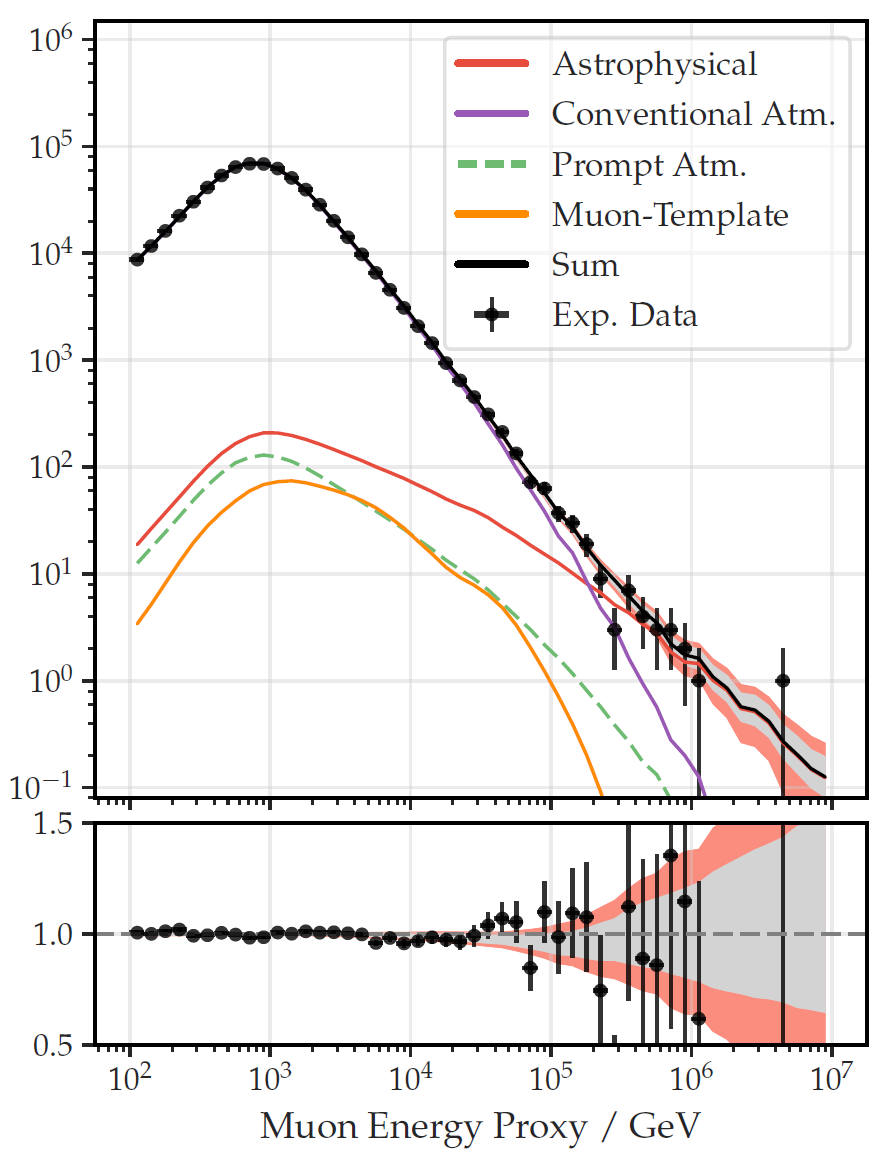
\includegraphics[width=\textwidth]{Ice_cube_flux_tot.png}
        \caption{Number of events per bin}
    \end{subfigure}%
    \begin{subfigure}[b]{0.5\textwidth}
        \centering
        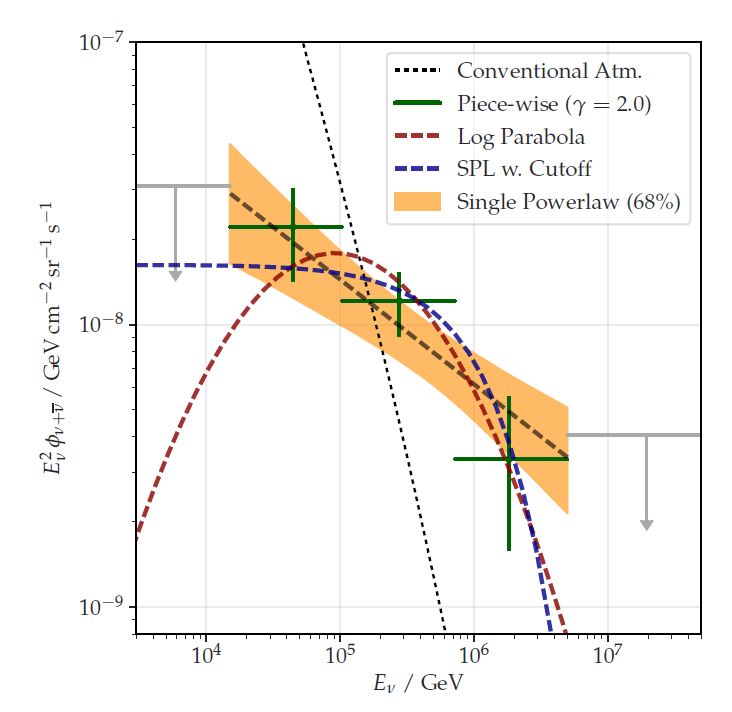
\includegraphics[width=\textwidth]{Ice_cube_flux_astro.png}
        \caption{Modeled Astrophysical flux}
    \end{subfigure}
    \caption{The diffuse flux of neutrinos as measured by the Ice Cube observatory. The y-axis on the left image is the number of events per bin.  The flux is separated into contributions from atmospheric neutrinos and astrophysical neutrinos. The right image is the model astrophysical flux as measured by ICE CUBE. Images taken from \cite{Abbasi_2022} }
    \label{fig:flux_neutrinos}
\end{figure}






\section{Active galactic nuclei}




Active Galactic Nuclei (AGNs) is an interesting field in astrophysical studies. 
Since their discovery, there has been rapid advancement in understanding these phenomena.
Today, AGNs are known to be among the brightest entities in the night sky,
but they only gained significant attention in the 1950s. 
This shift occurred with the arrival of new radio observations, which revealed a new type of quasi stellar
object through the discovery of Quasars.

Initially, these luminous objects, characterized by broad, 
unidentifiable spectral lines, were enigmatic to scientists in the early 1960s. 
However, with the identification of more sources and their optical parts, 
it became clear that these were not stars but a distinct class of celestial objects. 
Research done by M. Schmidt on of the emission lines from 
the Quasar 3C 273 opened the interpretation of these celestial objects. 
He found that the emmision lines of quasars were similar to hydrogen, but were redshifted by a factor of 0.158,
an exceptionally high value at the time \cite{Shields_1999}. Observations at the same time also revealed significant 
variability in quasar luminosity, suggesting that these objects were no larger than one light year across. 

These observations lead to the speculation of super luminous objects located very far away from earth. The problem was that such objects
had no reasonable explaination at the time. It was not until the mid 1960 early 1970s when modern cosmology was 
afoot that more of these issues were resolved.

Observation of the surrounding galaxy of AGNs with matching redshift and observation of gravitational lensing cemented 
the distances of these objects. In addition the modern view of black holes which had only been a theory in the 1950s came to
furition and the modern model of a AGN was born. This modern perspective views AGNs as supermassive black holes that
accrete matter from surrounding accretion disks. This accretion releases large amounts of energy and has also according to 
processes such as  the Blandford-Znajek process (1977), been shown to produce relativistic jets, when the black hole is rotating.

In the most recent times a landmark achievement was achieved in March 2021, when scientists associated with the Event Horizon Telescope project 
presented the first image of the supermassive black hole at the center of the Messier 87 galaxy, located 55 million light-years away.
This image, showing a bright ring surrounding a dark central region, aligns with predictions for an accreting supermassive black hole, 
reinforcing our understanding of these powerful cosmic sources.



\subsection{AGN structure and classification}


The modern view of AGNs is a unified model that combined different categories of powerful luminous objects viisble in the night sky.
These distinctions that astronomers made still
have value, but to understand an AGN it is important to get a picture of the modern structure of an AGN

An active galatic nucleous is defined as a galaxy containing a massive accreting black hole. This mass acording to \cite{Netzer_2015} 
is defined as $M_{BH} > 10^5 M_\odot$. AGNs aslo containt an Eddington ratio exceeding
the limit of $\frac{L_{AGN}}{L_{Edd}} = 10^{-5}$, where $L_{AGN}$ is the bolometric luminosity, and $L_{Edd}$ is the Eddington luminosity for a solar 
composition gas. These definitions are help constrain what galaxies might contain an AGN, f.ex it exludes the milky way 
by these criteria, but it failes to capture the full structure definition of an AGN. 
Therefore the structure of most AGNs will include several of the following components. 

\begin{itemize}
    \item A close rotational dominated accretion disc around the SMBH. The thickness defining this accretion flow will distinguish different AGNs. 
    One examples is an optiacl thin accretion disks that sometimes become advenction dominated.
    These flows will be referred to as radiation inefficient accretion flows(RIAF) due to the special nature of the disk.
    \item high density gas clouds that are said to be dust free moving at high velocities close to the black hole, in the so called broad line region(BLR)
    \item Low density gas clouds that move at lower velocities further away from the black hole in the so called narrow line region(NLR)
    \item A axisymmetric structure of dust that is responsible for the obscuration of the central region of the AGN. This is called the torus.
     It lies at a luminosity depended distance from the SMBH, but according to \cite{Netzer_2015} this is around 0.1 - 10 pc depending on the luminosity.
    \item A corona of hot electrons that is tohught to be responsible for the X-ray emission seen in AGN. This is thought to be located above the accretion disk. 
    \item A relativisitc jet that is powered by the accretion disk. This is not always present but is a common feature of AGNs.


\end{itemize}
The reader is directed to image \ref{fig:my_label} for a visual representation of the different components.


\begin{figure}
    \centering
    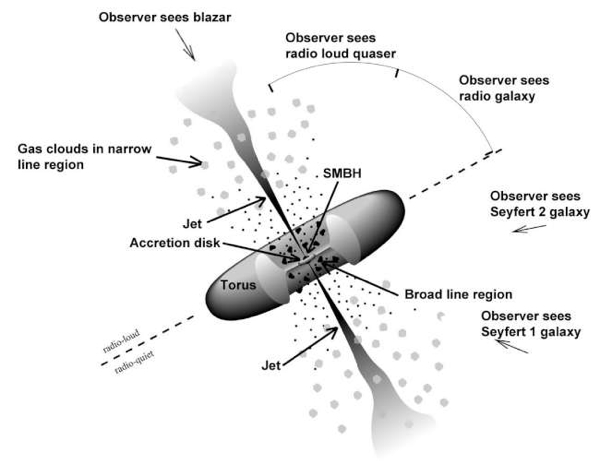
\includegraphics[width = 0.7\textwidth]{unified model agn.jpg}
    \caption{AGN unification}
    \label{fig:my_label}
\end{figure}

\subsubsection{Accretion disk}
An accretion disk is a natural consquence of the consveration of angular momentum. In the case for innfalling 
matter comming close to a super massiv black hole, the matter will have some angular momentum. This angular momentum would in a 
an ideal fluid orbit the black hole at some stable distance. Du to radative procesess, fluid viscosity and gravitational turbulence 
the matter will lose angular momentum and spiral inwards. This inward spiral will eventually allow the matter to fall onto the black hole. 
This process of insprial is what is called accretion and the forces acting on the matter to cause the inspiral 
will also in the same process heat it up to high energies causing it to radiate. This radiation is closly linked to the 
infalling matter that is accreted onto the black hole and one can express the total luminosity of the accretion disk as 

\begin{equation}
    L_{acc} = \eta \dot{M}c^2
    \label{eq:accretion_luminosity}
\end{equation}

Here $\eta$ is the efficiency of the accretion disk, $\dot{M}$ is the mass accretion rate and $c$ is the speed of light.

The efficiency of the accretion disk is a function of the spin of the black hole and the radius of the innermost stable circular orbit (ISCO).
The ISCO is a counter intruitve term in classical mechanics but in general relativity the maximum speed of a particle 
in addtion to a energy term when calculationg the orbit set bounds for how close a particle can be to 
a black hole without spiraling in. without going into to much detail the ISCO will be a solution of this equation based on the black holes mass and spin $a$

\begin{equation}
    6\frac{M}{r_{ISCO}}-8\frac{aM^(\frac{1}{2})}{r^{3/2}_{ISCO}}+3\frac{a^2}{r_{ISCO}^2} = 1
    \label{eq:ISCO}
\end{equation}
It is clear from \ref{eq:ISCO} that for a non rotating black hole the ISCO takes the radius of $6M$, the result obtained from the calculation using the swarzschild metric.


The accretion disk also has a bound for its maximum luminosity. As calculated for stars the Eddington
luminosity sets a maximum strength for the radiation pressure of the accretion disk. This is given as

Get sources!

\begin{equation}
    L_{Edd} = \frac{4\pi G M m_p c}{\sigma_T}
    \label{eq:eddington_luminosity}
\end{equation}

The heating of the accretion disc will lead to thermal radaition from the disc and this radiation will be
is proportional to the temperature of the disc. This temperature is radially dependent and if one assumse a opticlly thick but geometricly thin disk, also called a Shakura-Sunuaev disk
one can express the radative surface energy flux taken from \cite{BHradiation}(p. 106) as 

\begin{equation}
    \frac{dE}{dAdt}= F_{rad}(r) = \frac{3GM\dot{M}}{8\pi r^3}\left(1-\beta\sqrt{\frac{r_{ISCO}}{r}}\right)
\end{equation}

Here $\beta$ is a constant that relates the fraction of angular momentum captured by the black hole, and $r_{ISCO}$ is the radius of the innermost stable circular orbit. 
The temperature of the disk lie between $10^5 - 10^2$ K with emmision in the optical, UV to soft X-ray range. \cite{scholarpedia_accretion_discs}


\subsubsection{Corona and X-ray emission}
From high varying x-ray observations of AGNs it became indicative that there was a source of x-rays located close to the black hole. 
The most contemporary idea is that a corona of energetic particles is located above the accretion disk, and through inverse compton scattering
of the optical/UV photons that arise from the accretion disk produce the seen x-ray emission. 

Inverse compton scattering is the process of a photon gaining energy from a nearby relativistic particle. Due to the increase in efficiency 
of uppscattering a photon with an electron compared to a proton, the corona is thought to be dominated by electrons. The process is as follows

\begin{equation}
    e^- + \gamma \rightarrow e^- + \gamma 
\end{equation}

The reason of interest for this area is that the correlation between the produced x-ray luminsoity can be used to infer some lumunoisty of the more elusive 
particles UHECRs and neutrinoes. The reason for this is that the ingredients for this x-ray production is the same as for the production of UHECRs and neutrinos (charged praticles and photons). In addition 
the acceleration into the jet like structure of AGN needs a source of particles and the corona is a natural candidate for this.





%\subsubsection{Emmision lines}
%When a particle is photionized by the continuum radiation of a source it will emit a photon when it returns to its ground state. 
%This photon will have a specific wavelength that is determined by the energy difference between the two states.
%This wavelength is called the emmision line of the particle. When looking a dynamical systems with high velocities 
%the doppler shift of these emmision lines becomes important since it will affect the observed spectra of the source.

%https://lweb.cfa.harvard.edu/~pberlind/whipple/agn.html



\subsubsection{Broad and narrow lines region}

Broad emission lines in the case of AGN are formed from the high density gas clouds located close the the central black hole. The 
high density parameter is innferred from the fact that one only sees broad emission from permitted line transitions (f.ex hydrogen Lynman and Balmer,
iron II, and magnesium II). High densities allow for collisional de-exitation and in doing so prohibits so-called forbbiden transitions.
The broadaning is an indictation that these gas clouds are moving at  huge velocities around the massive objects. This implies that they are located close to the black hole and recive the name the broad line region

Narrow emission lines are on the other hand formed in low density gas clouds. The low densities are inferred from the fact that one sees
both permitted and forbbiden line transitions. They are narrow lines due to their velocities being substantially lower than the inner most gas clouds, and from here are thought to be located further away from the black hole, in the narrow line region. 


\subsubsection{dust torus}
%https://www.sciencedirect.com/science/article/pii/S0032063315000483#:~:text=This%20model%20proposes%20that%20all,collimating%20the%20radiation%20that%20escapes

The dust torus is a structure of dust that is tought to be located quite close to the black hole (0.1 - 10 pc). The main argument for the existance of this structure is the obscuration of the central region of the AGN. This obscuration 
is part of the unfiication scheme of AGNs and was backed by the detection of polarized broad lines in AGNs with their central core obscured. This polarization is what we would expect if some dust was obscuring the central region, since the only light one sees is 
the light that is scattered into our line of sight \cite{MASON201597}. Further studies on the dust torus has also revealed that the torus is not unifrom but clumpy and quite dynamic with both in and outflows of matter depedning on the state of the central engine \cite{MASON201597}. 




The unified model of AGNs 


mabye write about thermal radiation from dust torus


\subsubsection{Jets}

A jet is a highly collimated outflow of plasma. The origin of the plasma is thought to be the accretion disk and the hot corona above it. These regions who have a high density of charged particles will  under the infulence of a magnetic field be accelerated and collimated into a jet like structure.
The energy mechanism which powers the jet is not fully understood but the most prevalent theory is the Blandford-Znajek process. It says that the roation of the accretion disk  induces a magnetic field which will interact with a rotating balck hole, effectivly extracting energy from the black hole and supplying it to the jet. 
The jet structure extends far beyond the local area of the AGN maintaining a stable configuration over these distances. The classification of these jets are usually divided into two groupd, FRI and FRII. They are differentiated by their luminosity where FRI jets are less luminous and have a more diffuse structure while FRII jets are more luminous and have a more stable structure reaching further out. \cite{walg2013relativistic}.
Beyond the energy and their structure the jets are also notable for their emission of non-thermal radiation such as synchrotron and inverse compton radiation. They are also thought to be a possible source of UHECRs and neutrinos.


Write about shock structure
write about non thermal radiation
Jet acceleration?, acceleration before jet, cooling effects



section radiation




\subsection{Types of AGNs}

https://astrobites.org/guides/galaxy-and-agn-types/

Before the unification of the AGNs astornomers named the pusseling objects based on their observational properties. These 
names are still used to this day and are somewhat usfull since their observational properties are important parameters for further study. 
The different classification are important in understanding which objects could have the potential to produce the different oberservables one 
looks for in the night sky. There is a lot of talk around AGNs being possible sources for ultra high energy comsic rays (UHECRs) and neutrinos.
This is yet to be comfirmed, but the theoretical framework for the neceassary particle acceleration is there. therefore is seems appropriate to
discuss the different types of AGNs and their observational properties.

\textbf{Type I and II AGNs}:
One distinguishes type I and type II AGNs based on the presence of broad emission lines. In other words this distinction is
a matter of a visible nucleous or not. Type I refers to sources whose nucleus is exposed to the observer and whos spectrum
has both narrow and broad emmision lines. Type II refers to sources whose nucleus is obscured by a torus and therefore only has narrow emission lines.

\textbf{Blazars}:
The most extreme class of AGN. These sources are distinuished by their relativistic jets that are pointed towards the observer. 
This jet produce both synchrotron and Inverse Compton gamma rays and are extremyl varaible over short timescales. The
emission is also highly polarized. Often and including in this paper one divides blazars into subgroups based on the 
emission lines. The two most common are BL Lacs and Flat spectrum radio quasars (FSRQs). The difference between these two is the
presence of broad emission lines. BL Lacs have no broad emission lines while FSRQs do.

\textbf{Radio galaxies}:
As the name suggest these sources are very bright in the radio band. The usally refer to AGN viewed edge on, where the
torus might block the emmisions from the accretion disk. The oriantation of Radio galaxies give way for strong 
synchrotron radiation, and they are often used to study the jet structure of AGNs.

\textbf{Seyfert galaxies}:
Spiral galaxies that have a bright nucleous. They are bright in the optical band and have a smaller active region 
than radio galaxies. They are often divided into two groups Seyfert I and Seyfert II where the distinction comes from type I and II. 
They also show quite high variablitlty indicating a small emmiting region. 

%https://iopscience.iop.org/article/10.1086/305813/fulltext/37493.text.html#:~:text=,line%20time%20delays%2C%20or%20lags


All these different distinctions are a help in understanding what processes one might be observing. The different
dominant bands indicate different procesess being in our line of sight, and by considereing the modern structure of 
AGNs one can then try to determine the underlying dynamics.  


\section{ Luminosity functions}
In this section we will discuss the use of luminosity functions to characterize the populations of different AGNs in time/volume and energy. 
A luminosity function is a function that describes the distribution of objects by their luminosity and their comvoing volume element for a population of celestial sources,
such as galaxies or quasars. It is a powerful tool for understanding the properties and evolution of 
these objects, as well as the larger-scale structure of the universe. 
%The function describes how a population varies based on luminosity but also crucially on its comoving volume element. 
 We usually talk about the differential luminosity function given as
\begin{equation}
    \frac{d\Psi(L,z)}{dL} = \frac{d^2N(L,V_c(z))}{dLdV_c(z)}
\end{equation}

%The quantity of interest is now a number density which can be very useful in deriving observed flux of different objects here on earth. 
On also can change the differential of the comoving volume into a term only depending on the redhsift assuming the source population is isotropic and by mulitplying with the differential comoving volume element.

\begin{equation}
    \frac{d^2N(L,V_c(z))}{dLdV_c(z)}\frac{dV_c(z)}{dz} = \frac{N(L,z)}{dLdz}
\end{equation}


Several articles express the luminosity function in base $10$ logarithm and we note the conversion between the two. 

\begin{equation}
    \frac{d\Psi(L,z)}{dLog(L)} =  \ln (10)  Lx \frac{d\Psi(L,z)}{d(L)}
\end{equation}


The luminsoty function(LF) is a theoretical tool, but in order to determine the luminosity functions one usally seperate the function into two terms. 
One takes the local luminosity function at $z=0$ and then multiply it with a redshift evolution function. These evolutions functions
are varying from survey to survey, but in general one has two main classes. 
The different classes are seperated on how the evolution term is added to the local LF and is determined on what fits the evolution the best. 
The pure density evoltuion (PDE) model evolves the local density function while the pure luminosity evolution (PLE) model evolves the local luminosity.
The evoution is better represented by its equations and is given as 

\begin{equation}\frac{d\Psi(L,z)}{d(L)} = 
    \begin{cases}
        \frac{d\Psi(L/e(z),z=0)}{d(L)} \quad (PLE)\\
        \frac{d\Psi(L,z=0)}{d(L)}e(z) \quad (PDE)\\
    \end{cases}
\end{equation}

The PLE and PDE models sometimes fails to capture the evolution of the luminosity function. Therefore modern 
LF might use a modified version. This will be come more clear in the next section.

\subsection{X-ray LF}

\begin{table}
\centering
\title{Parameter values for the X-ray luminosity functions}
\begin{tabularx}{\textwidth}{|l|XXXX|XXXXX|}
\hline

& \multicolumn{2}{c}{\textbf{LF params}} &&&  \textbf{Evolution params} &&&&\\

\textbf{Model} & $A$ & $L_{star}$ & $\gamma _1$ &  $\gamma _2$  & $v_1$ & $v_2$ & $z_c$ & $L_c$ & $ \alpha$\\
\hline
SLDDE RG & $8.375^a$ & $2.138^b$ & 2.15 & 1.10 & 4.00 & -1.50 & 1.90 & $3.981^b$ & 0.317  \\

AMPLE-Blazar & $1.379^a$ & $1.810^b$ & -0.87 & 2.73 & 3.45 & -0.25 & & &  \\

AMPLE-FSRQ & $0.175^a$ & $2.420^b$ & -50.00 & 2.49 & 3.67 & -0.30 & & &  \\

APLE-BLlac & $0.830^a$& $1.000^b$ & 2.61 & &-0.79& & & &  \\
\hline
\end{tabularx}
\caption{X-ray LF parameters, $a)$ normalised by a factor of $10^{-7}$, $b)$ normalised by a factor of $10^{44}$}
\label{tab:xray_lf}
\end{table}

\begin{table}
    \centering
    \begin{tabular}{ll}
    \hline
     Model Name   & Luminosity Range (Log(L))  \\
    \hline
     SLDDE\_RG     & 42 - 47            \\
     AMPLE\_Blazar & 44 - 48.5          \\
     AMPLE\_FSRQ   & 46 - 48.5          \\
     APLE\_BLlac   & 44.5 - 48.5        \\
    \hline

\end{tabular}
\caption{Luminosity range for different models}

\label{tab:lum_range}

\end{table}


%One way of calculating the neutrino flux of AGNs is based on their connecting with x-ray radiation. 
%Therefore in some literature, it is of interest to define the x-ray luminosity function for AGNs.

For a given type of celestial objects, different bands will be more important than others, but for populations such as AGNs
 the x-ray luminosity from these sources are of interest. 
Therefore several studies attempt to describe the luminosity functions of these sources through the use of the x-ray band. 

In the following analysis I will look at the x-ray luminosity functions of several classes of AGNs; Radio galaxies, Blazars alone and with the additonal subdivision into FSRQs and BLlacs, and Seyfert galaxies. In addition to this 
a study by \cite{Ueda_2014} also look at the total evolution of AGNs which is interesting. The luminosity functions are collected from three papers \cite{Ajello_2009} and \cite{Silverman_2008}, and \cite{Ueda_2014} and their form is explained below.

\textbf{The local luminosity function}:
The local luminosity function is the luminosity function at $z=0$ and is the starting point for the evolution of the luminosity function.
The most simplest form of the local luminsoty function is expressed in \cite{Ajello_2009} and is given as a power law.

\begin{equation}
    \frac{d\Psi(L,z=0)}{dL} = \frac{A}{L_x} \left( \frac{L_x}{L_*}\right)^{1-\gamma_2}
\end{equation}

This functional form has the fewest parameters, but has the disadvantage of not being able to capture all the details of the observed local luminosity functions.
For that reason a more complex local function is needed which was proposed in \cite{Ueda_2003} and is described by a double power law.
The functional form of the double power law is as follows.


   
\begin{equation}
    \frac{d\Psi(L,z=0)}{dL} =  \frac{A}{\log(10)} \frac{1}{L_x} \left( \left( \frac{L_x}{L_*} \right)^{\gamma_1} + \left( \frac{L_x}{L_*} \right)^{\gamma_2} \right)^{-1}
\end{equation}

The double power law introduced a break luminosity $L_*$ which is the luminosity where the slope of the luminosity function changes.


\textbf{Evolution factor}
In addition to the local LF one also considers the evolution factor denoted $e(z)$. This factor captures the observed evolution of these objects and is the second part of the total luminosity function.

Again for the simplest evolution with the fewest parameters a power law is used.
 $$
e(z) = (1 + z)^{v_1 }
 $$


  
Certain situations necessitate a more detailed approach to the redshift evolution. 
 As detailed in \cite{Ajello_2009}, a modified evolution is frequently employed. 
 This adaptation transforms the conventional Pure Luminosity Evolution (PLE) and Pure Density Evolution 
 (PDE) into their modified counterparts, namely Modified PLE (MPLE) and Modified PDE (MPDE).
It is within these modified frameworks that a dependence on redshift $z$ emerges in the exponent,
providing a more nuanced understanding of the evolutionary processes involved. It is given as

$$
e(z) = (1 + z)^{v_1 +v_2 z }
 $$



 To expand further as described in \cite{Ueda_2003} the evolution factor of the luminosity function is not always a simple as a modified power law only dependent on the redshfit $z$.
For some sources a more complex evolution is needed. In \cite{Ueda_2003} they use a double power law to better fit the data where 
 the evolutions is now not only dependent on the redshift but also on the luminosity. This then recvies the apt name as a luminosity dependent density evolution (LDDE) since it is a modified version of a (PDE)


 \begin{equation}
    e_z(z, L) = 
    \begin{cases} 
    (1 + z)^{v_1} & \text{if } z \leq z_*(L) \\
    e_z(z_*(L), L) \times \left( \frac{1 + z}{1 + z_*(L)} \right)^{v_2} & \text{if } z >  z_*(L)
    \end{cases}
 \end{equation}

 with $z(L)$ being defined as

 \begin{equation}
    z_*(L) = 
    \begin{cases} 
    z_c \left( \frac{L}{L_c} \right)^\alpha & \text{if } L \leq L_c \\
    z_c & \text{if } L > L_c 
    \end{cases}
 \end{equation}


 The expansion of the parameter space allows for easier fitting to the observed data, but comes of course with an increase in complexity and possible overfitting. 


Armed with the functional form of the total luminsoity function one can now fit the parameters to the observed data. This is done in \cite{Silverman_2008} and \cite{Ajello_2009} and their 
model name is a comination of the soruce paper (S, A), the type of model it desribes (PLE, MPLE, LDDE) and the object in question. The parameters are then fitted to the data using a maximum likelihood method and the observational data of several x-ray surveys, see the cited papers for more information.
One can see the parameters for the different models in table \ref{tab:xray_lf} and the luminosity range for which the different models are valid in table \ref{tab:lum_range}.





\section{Evolution}
In this section we will be using the different luminosity functions from the previous section to calculate the evolution of the different classes of AGNs. 
This evolution illustrates the different distribution one can expect from our different classes accros luminosity and redhsift, highliting their evolution in time and energy.
%By looking at the different trends for the different type of distributions one can observe the evolution and energy distribution of the different classes of AGNs. 


\subsection{AGN evolution}
With the luminosity function one can calculate the evolution of the different classes of AGNs.This evolution is interesting because it will 
illuminate what could be the expected trend of different oberservables such as UHECRs and neutrinoes produces in the same crucible.
In this section we will be looking at the different distribution of the different classes of AGN 
mentioned above, by using the X-ray luminosity function. 


\subsubsection{Luminosity distribution}
 
For the different classes discussed one can integrate the differntial luminosity function to retrive the Luminosity distribution of each 
object. This distribution highlighst the difference over emmitting power and therefore are important for us to be able to distinguish the most powerfull 
sources and their prevelance. One calculates the Luminosity density by mulitplying the class specific luminosity
function with the differential comoving volume and integrating over the relevant redshift bin. By seperating it into
bins of redshift one will illuminate the number evolution in time of these objects. It is important to note 
that the evolution beyond the given luminosity range is not known and therefore the distribution is not complete. And deducing continued evolution
can be done but must be taken with a grain of salt. The number of objects these functions are built upon are not very numberous and therefore
the error bars are quite large, especially in the edges. 




\begin{equation}
    \frac{dN(L)}{dL} = \int_{z_{\text{min}}}^{z_{\text{max}}} \frac{\Psi(L, V(z))}{dL} \frac{dV(z)}{dz} dz
\end{equation}


\begin{figure}
    \centering
    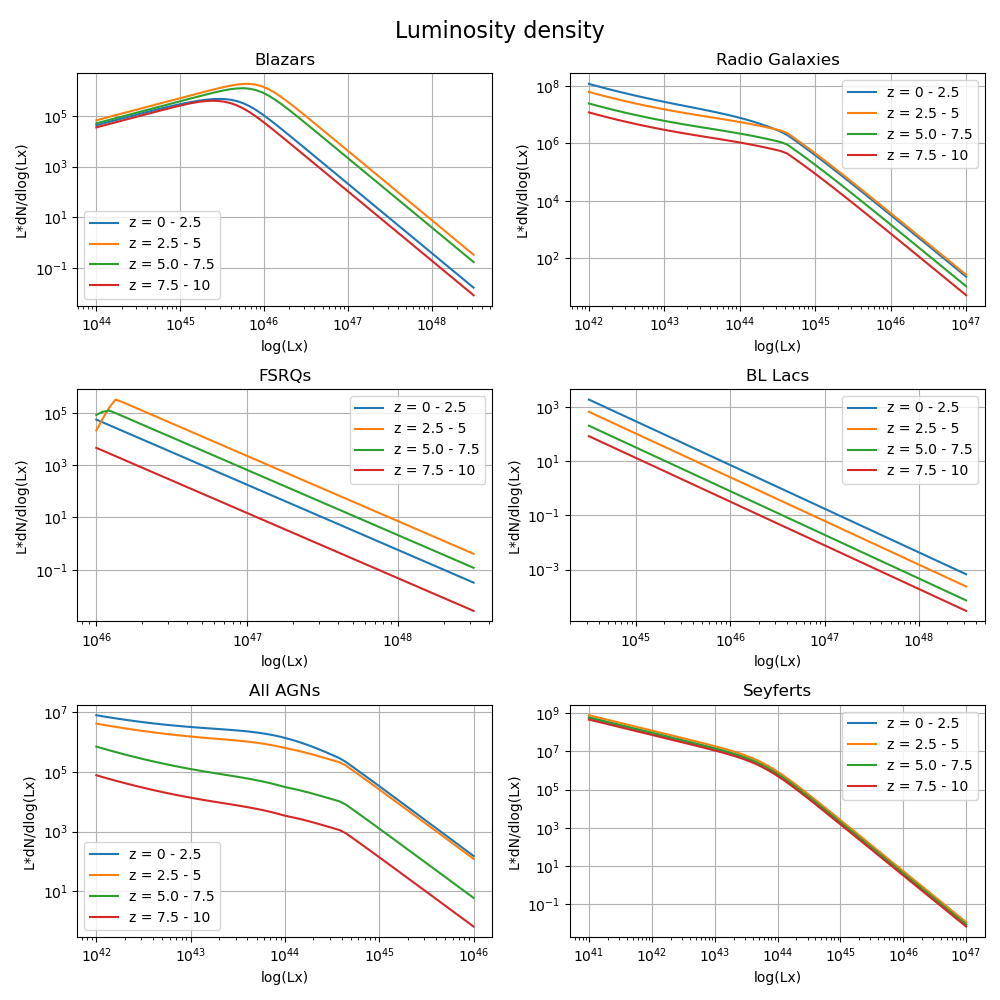
\includegraphics[width = \textwidth]{new_plots/Luminosity density.png}
    \caption{Luminosity density for the four different classes of AGNs. The different classes are defined in the title as well as the chosen LF model.}
    \label{fig:LD}
\end{figure}

In figure \ref{fig:LD} one can see the luminosity density for the four different classes of AGNs. The distribution are 
seperated into four bins of redshift ($0<z<2,2<z<4,4<z<6,6<z<8$). %
%This is done to illuminate the evolution of the different classes at different epochs
  
For the blazar population in the top left of image \ref{fig:LD} one sees a clear break around $10^{46}$ erg/s. This break indicate that there is a distribution
around this value and that the most common blazar will be found around this energy level. The distribution also shows a clear evolution in time. wheras the earliest epoch
and the current epoch both have the fewest number of sources. In addition the middles epochs have a larger population at higher energies meaning a much energy output in these times. 

For the FSRQs and for the BL Lacs one sees a different distribution. Where one sees more sources as we go to lower energies. The break luminosity for FSRQs 
is very close to the edge of the luminosity range and is almost not visible. The Bl Lacs on the other hand do not have a break 
due to their representation as a simple power law. They have a clear difference in what epochs contributed most where the FSRQs follow the blazar population by having a larger population at the 
middle epochs. The bl lacs on the other hand have an increasing population over all energy bins as we go to lower redshifts.

For the Radio galaxy population one sees a broken powerlaw distribution. Here the distribution has a break at $10^{45}$ erg/s and then continues to 
decrease but with a harder slope. The figure also shows an increase in population of the lower energies but a stagnation in the higher energies. 
 %To explain the hardening of the slope one might turn to classification issues with AGNs but it is not clear.


\subsubsection{Density distribution}

In addition to the luminosity distribution one can also calculate the number density of the different classes of AGNs. This is done by integrating the
differential luminosity function over all luminosities. This will illuminate the evolution of the different classes of AGNs in terms of redshift. The integral is given as

\begin{equation}
    \frac{dN}{dz} = \int_{L_{\text{min}}}^{L_{\text{max}}} \frac{\Psi(L, V(z))}{dL} \frac{dV(z)}{dz} dL
\end{equation}

Here again we seperate into luminosity bins in order to see the evolution seen in the previous chapter. This might seem redundent but
it gives one a stronger intution of the number of objects that are most common at which epoch, and their luminosity. 





\begin{figure}
    \centering
    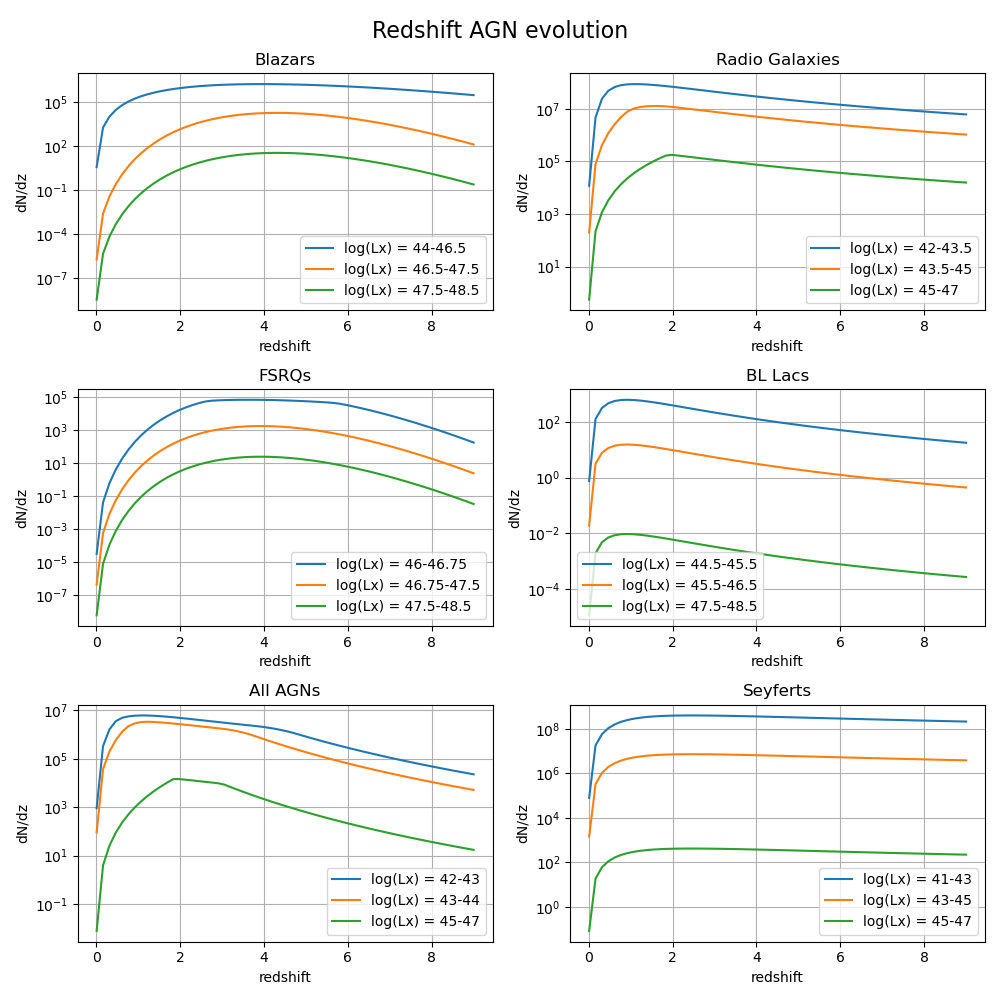
\includegraphics[width = \textwidth]{new_plots/Redshift AGN evolution.png}
    \caption{Number evolution in terms of redshift for the four different classes of AGNs. The different classes are defined in the title as well as the chosen LF model.}
    \label{fig:ND}
\end{figure}



In figure \ref{fig:ND} one sees the number evolution of the different classes of AGNs. The evolution is seperated into three bins of luminosty each calculated in the same manner as \cite{Jacobsen:2015mga} which did the same analysis.

For the blazar population in the top left of image \ref{fig:ND} one sees a clear trend with a top point around redshift $z=5$. 
This is then the epoch where most blazars are present, and the evoltion is more clear for higher energies. This is simialr to what we saw for the luminosity distribution and highlights the fact that blazars dominated earlier epochs and are in decline. 


For the FSRQs the evolution is quite linked to the blazard population. This is expected since FSRQs and BLlacs are thought to be 
sub groups of the bigger blazar group. The evolution also peaks around redshift $z=5$ but is less uniform over time. There is a bigger drop 
in numbers in the earlier and more recent epochs. For Bllacs the distribution is very different. Here the peak comes more aorund redhsift $z=2$ and then drops of quite rapidly for older epochs.
This is interesting since it might indicate a change in type of AGN that is created. Why does one see less broad band emmision lines from blazars as these plots indicate? 

For the radio galaxies the trend is similar to the Bllacs. The peak of the time evolution is at more recent epoch ($z=1$) and the peak is 
luminosity dependent. The peak of the most luminous radio galaxies are at higher redshift than the less luminous ones. This shift indacates a decline in these super luminous objects and they are being replace by less powerfull objects. 
%In addition from source .... one can find
%the evolution comparable to the evolution of the star formation rate. This is interesting since it might indicate that the two are linked.


The representation of these objects can also be shown by their density distribution. By simply dividing the total number density by the comoving volume one can
find the density of these objects in the universe. By looking at figure \ref{fig:DD} one can see the density distribution and the effects this has on our interpretation of these objects.

The evolution is similar to that of the total number evolution, but one highlights the biggest difference between the groups. That one groups namely the Bllacs and the radio galaxies
are increasing in density when looking at lower redshifts and the other two groups are decreasing. This is a very interesting result since it might indicate that the two groups are 
a product of a different conditions in the universe, for example the totalt density of matter. In addition the decline in higher luminosty objects of both blazars and RG is curious since one would only expect the 
super massive black holes that produce these objects to increase in size since the beginning of the universe and from equation \ref{eq:eddington_luminosity} this evolution allows for higher stable luminosities. The explaination is probably related to equation \ref{eq:accretion_luminosity} 
and realising that the accretion rate is not constant and is dependent on the amount of surrounding material to accrete.  



\begin{figure}
    \centering
    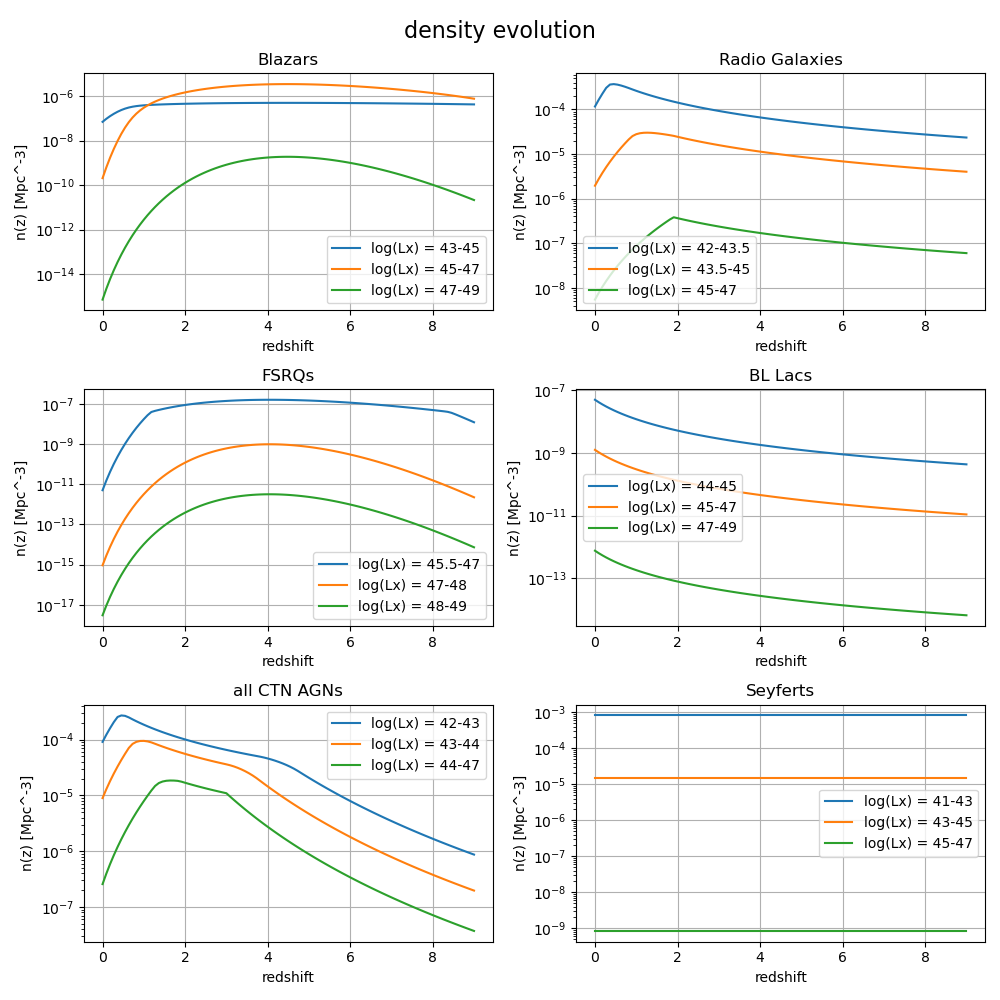
\includegraphics[width = \textwidth]{new_plots/Redshift density evolution.png}
    \caption{Density distribution for the four different classes of AGNs. The different classes are defined in the title as well as the chosen LF model.}
    \label{fig:DD}
\end{figure}



\subsubsection{Expected luminosity}
From the luminsity function one can also calculate the exptect luminosity of an source class at different redshift. This is important since it will directly relate to the 
power output of the different epochs and from this one can calcualte an expected emmisitivty of the different classes of AGNs. 
The expected luminosity of each group can be calcualted with the following formula. 

\begin{equation}
    \langle L \rangle = \frac{\int_{L_{\text{min}}}^{L_{\text{max}}} L \frac{\Psi(L, V(z))}{dL} \frac{dV(z)}{dz} dL}{\int_{L_{\text{min}}}^{L_{\text{max}}} \frac{\Psi(L, V(z))}{dL} \frac{dV(z)}{dz} dL}
\end{equation}

The different luminosity ranges are the same as before and are given in table \ref{tab:lum_range}. The results are shown in figure \ref{fig:EL}.
In addition a simple multiplication of the density distribution and the expected luminosity will give the expected emmisivity of the different classes of AGNs. This is also shown in figure \ref{fig:EL}.

\begin{figure}
    \centering
    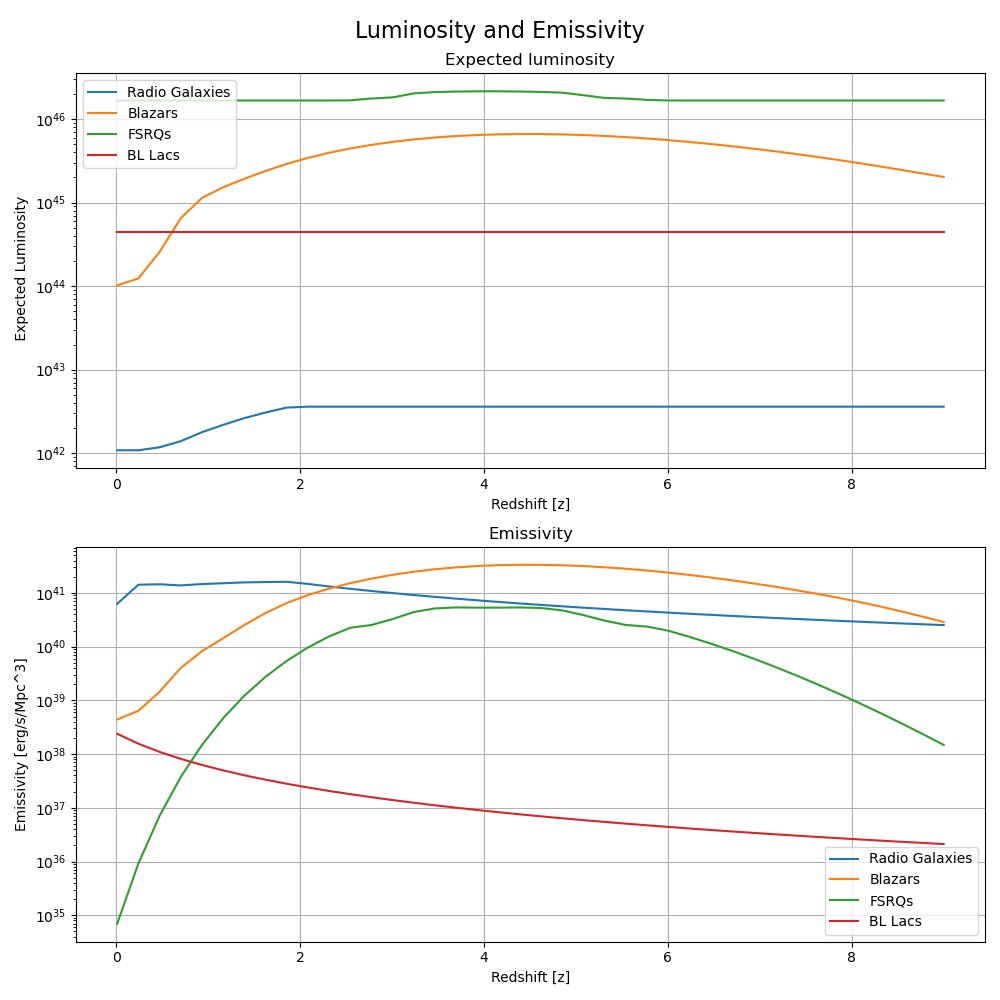
\includegraphics[width = \textwidth]{Luminosity and Emissivity.png}
    \caption{Expected luminosity and emmisivity for the four different classes of AGNs. The different classes are defined in the title as well as the chosen LF model.}
    \label{fig:EL}
\end{figure}

The expected luminosity shown at the top is a great reminder of the different classes. Here one sees that FSRQs are inndeed the most luminous part of a blazar AGN and 
that they represent some of the most luminous objects in the universe. The trend for FSRQs is also very flat with a small bump at the middle epochs. showing that the FSRQs are not becoming dimmer but less numerous.

The Bllacs on the other hand are not as luminous as the FSRQs but are still very luminous. 
The trend for the Bllacs is a very flat evolution indicating that the produced Bllacs although fewer at earlier epochs are still 
of similar magnitudes.

The group with the biggest varaibility in expected Luminosity is the blazars. Here one sees a curve over the epochs with a peak around redshift $z=5$. 
This indicates that the produced blazars in newer epochs are less luminous on averge. A similar results obtained from the luminsoity distribution in figure \ref{fig:LD}.
%The evolution of the expected luminosity might be indicative of a badly defiend gorup of objects since one usually distinctions objects based on their luminosity.

The radio galaxies are the least luminous of the four groups and have a very flat evolution. This is expected since the radio galaxies are not as luminous as the blazars.

The emmisivity shown at the bottom in figure \ref{fig:EL} shows a more intersting evolution. The figure shows the output of energy per unit volume per unit time. In other words 
how much energy these objects are producing and by extension which objects would be relevant at different epochs due to their dominance over the others.
The most interesting point is around redhsift $z=2$ where the emmisivity of the radio galaxies overtake the dominant blazars. This change would in theory make
a big splash in the observables here on earth should these objects be the origin of the UHECRs and neutrinos. The most interesting part is that a higher luminousity in x-ray would 
reasonably increase the luminosity of neutrinos and UHECRs, but due to energy loss, UHECRs can't be produce far away from earth. By speculating that they are produced in the same source one should expect a 
higher local energy flux of neutrinoes since more should be created in blazars whih would reach us. 


\section{Energy arguments}
\subsection{UHECRS emmisivity}
With the calculated emmisivity for the different groups there is now possibility to look from an energy budget viewpoint into the possibility of AGNs being the origin of UHECRs. The 
reasoning is quite simple but in order for the AGNs to be the origin of UHECRs they must be able to produce the necessary emissivity. 

From our own calcuation in \ref{sec:emmisivity} the energy density of UHECRs is given as $7 \cdot 10^{44}\frac{erg}{Mpc^3yr}$ this was calcuated from the observed flux of UHECRs from the Pierre Auger observatory \cite{thepierreaugercollaboration2017pierre}.
This emmisivity is very interesting due to the energy loss a UHECR will experience when travelling through the universe. We used the energy loss to somewhat arbritrarly limit the distance a UHECR could be produced from.
Therefore we must choose the emmisivity of our sources from similar distances since it may change. By looking at the emmisivity at very close redshift one can comapre the two values. The redshift chosen for comparison is $z=0.01$ which is  very close to our local area. %smoewhat in the middle of the distance limit of our UHECRs ($z= 0.2$). 
To calculate the emmsisitity of our sources one takes the density of these sources at the desired redshift and multiplies it with the expected luminosity at the same redshift.


%In order to estimate the sources of these UHECRs and based on the limit of how close an UHECR could be produced to earth one can calculate the emmisivity needed to produce these UHECRs.
%By estimating the emmisivity produced from our sources at a very low redshift (i.e $z=0.01$) one can then calculate emmisitivty of our sources and compared to the required emmisivity.

The resutling figure is shown in figure \ref{fig:UHECR}.

\begin{figure}[H]
    \centering
    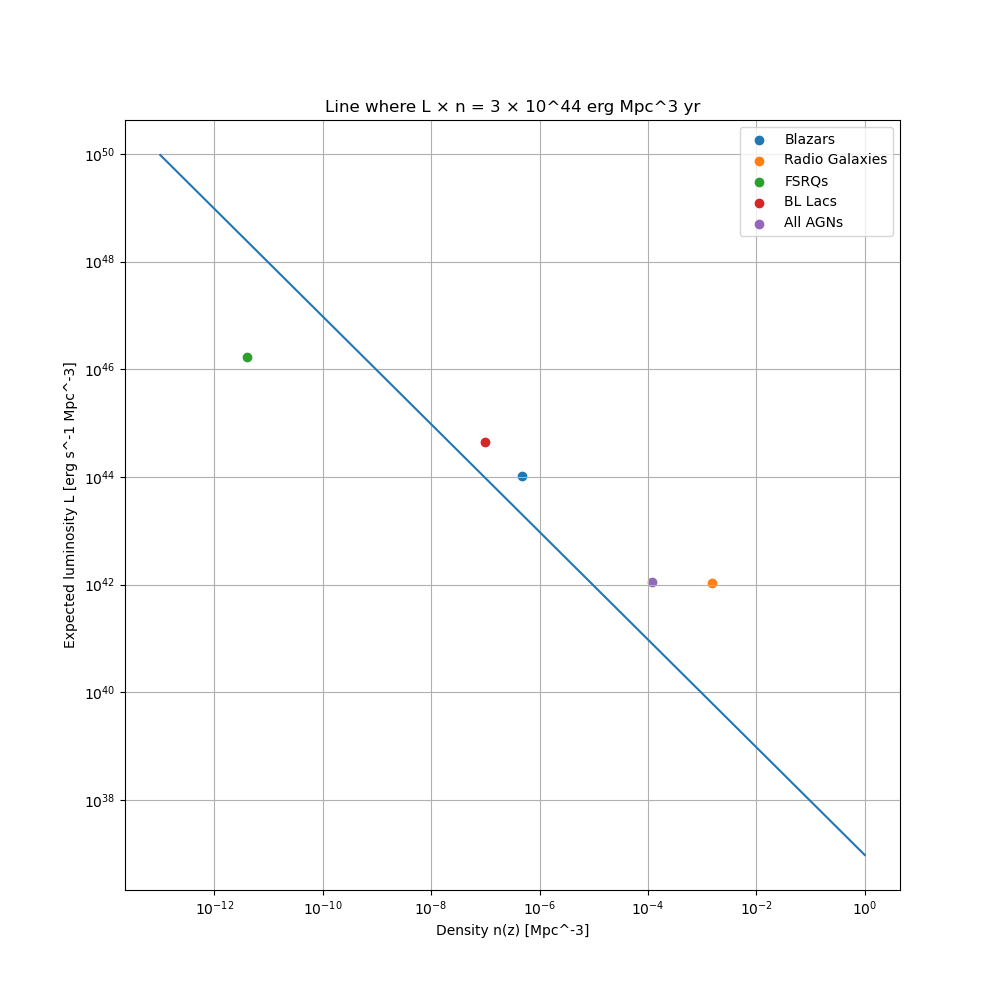
\includegraphics[width = \textwidth]{L_n_line.png}
    \caption{UHECR emmisivity for the four different classes of AGNs.}
    \label{fig:UHECR}
\end{figure}

The figure shows that almost all classes produce enough energy in X-rays in order to produce the required emmisivity. The only exception is the FSRQs where the number
density limits the required emmisivity. This result is a fine indication that AGNs could be the origin of UHECRs. However this is a very crude estimate and the
the correlation between X-ray luminosity and UHECR luminosity is not well defined and might include intrinquities that are not accounted for.

\subsection{Neutrino emmisivity}
In a similat fashion we calcualted the local emmisivity for the neutrinos in section \ref{sec:emmisivity}. The result was $1.2 \cdot 10^{45}\frac{erg}{Mpc^3yr}$ which is a factor 10 higher than for UHECRs.
In the calcualtion the neutrino flux was taken from the IceCube observatory \cite{Abbasi_2022} and the energy range was taken to be $1TeV - 10PeV$ which should be the astrophysical neutrino flux.
the difference from the UHECR flux is the energy loss and our emmiting area is now the whole universe. In order to reach a comparable emmisivity one must therefore take an average of our sources over the whole universe.
The  resulting figure is shown in figure \ref{fig:neutrino}.

\begin{figure}[H]
    \centering
    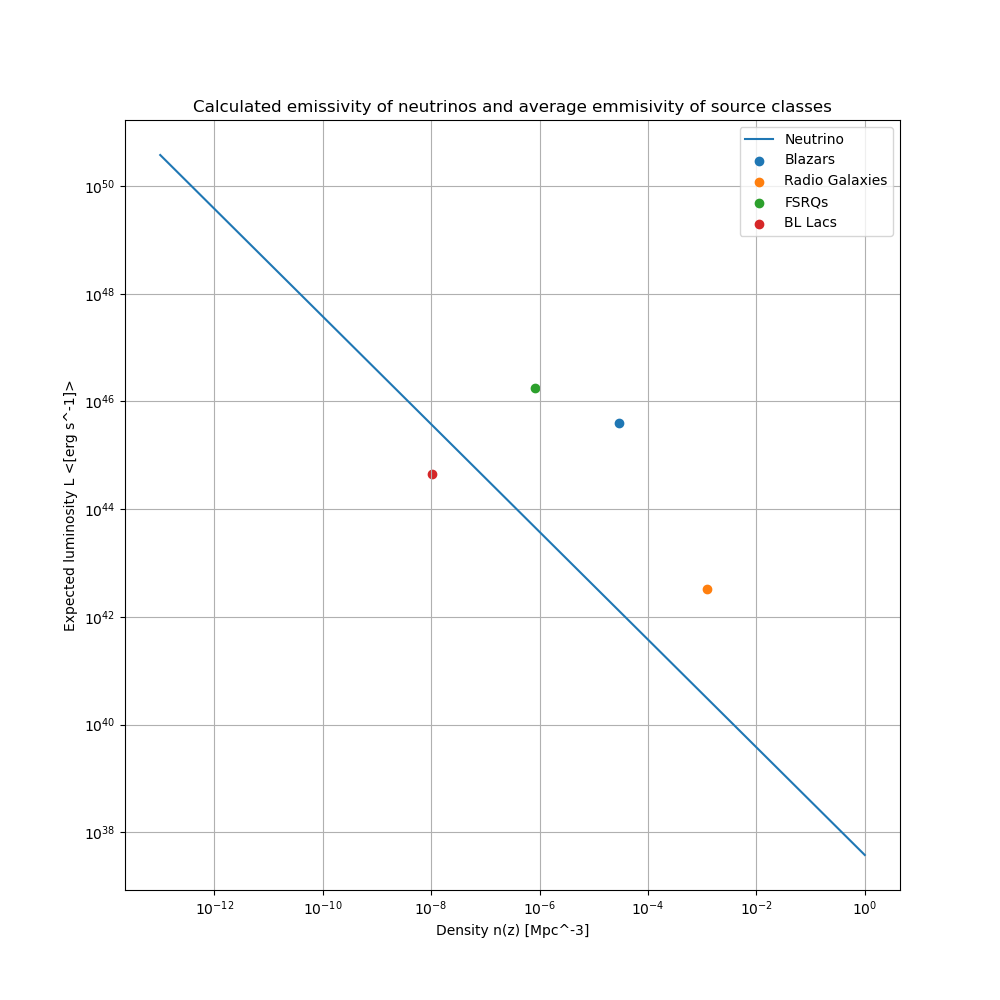
\includegraphics[width = \textwidth]{L_n_neut_calc.png}
    \caption{Neutrino emmisivity for the four different classes of AGNs.}
    \label{fig:neutrino}
\end{figure}

This figure shows that the neutrino flux can be produced by all classes except 
the BL Lacs. This is an effect of the avereging since the BL lacs have a postive evoultion.
 The opposite are the FSRQs who now are able to produce the required emmisivity.

The averaging proceedure does not take into account that the neutrino flux accutally loses energy when it travels throught the universe which should weigh earlier source less, and we can do better than a crude average. 
From \cite{Palladino_2020} one can define the diffuse neutrino flux as a transfer function which takes into account the energy loss of the neutrinos. This transfer function is given as

\begin{equation}
    \frac{d\phi_\nu}{dE_\nu} = \int_0^{z_{max}} \frac{D_H}{E(z)} \frac{L(E_\nu (1+z))}{(1+z)^2} \rho(z) dz
\end{equation}

here $D_H$ is the Hubble distance, $E(z)$ is the function defined in section \ref{sec:comoving_distance} , $L(E_\nu (1+z))$ is a power law representing the neutrino flux at the source, when integrated reproduces the source luminosity, and $\rho(z)$ is the number density of our sources at redshift $z$.
with this function we can calculated the expected diffuse flux of neutrinos from our sources. The result is shown in figure \ref{fig:neutrino_diffuse}.
\begin{figure}[H]
    \centering
    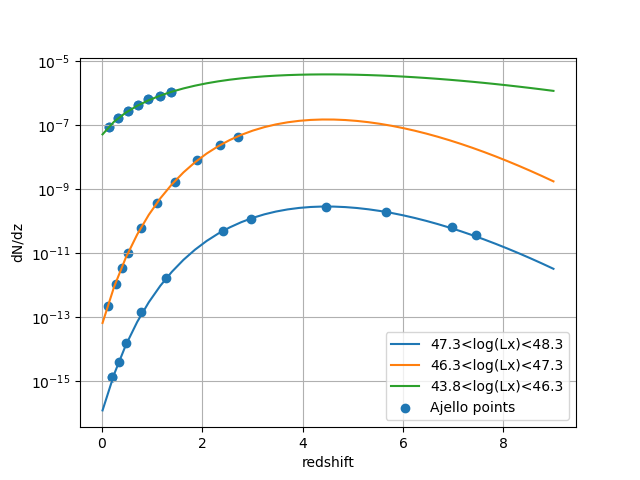
\includegraphics[width = \textwidth]{new_plots/Blazar_test_fit.png}
    \caption{Diffuse neutrino flux for the four different classes of AGNs.}
    \label{fig:neutrino_diffuse}
\end{figure}

what one sees here is the same result from our crude average. The FSRQs are now able to produce the required emmisivity and the BL Lacs are not. The result has several flaws. Firstly the estimated power law of neutrinos is the same as for the observed ICE CUBE diffuse flux. This is a very arbritrarly chosen power law and does not represent any of the parameters that might be included into the production of neutrinos except the x-ray luminosity. 
The remedy for this is to define a bottom up approach for the nuetrino prudction more carefully based on the x-ray luminosity. By doing such an approach one can begin to test our different models for the neutrino production and see if they are able to produce the observed diffuse flux. 
This is however outside the scope of this paper and will be left for future work.
The fact that all sources are overshooting the observed neutrino flux would be a problem if we had a more constrained solution. Any solution that overshoots will not be the source since it is not what we observe, but in our case 
our solution rest on the fact that the neutrino luminsity is equal to the x-ray, an assumition easily broken and without nuance. Therefore the only concrete conclusion one can draw from this is that the neutrino flux can be produced by our AGNs since they are able to produce the required emmisivity.
From several papers one can also include the dipole moment arguments which introduces a required density of sources to produce the observed isotropy of neutrinos. This would be a problem for our more obscure sources FSRQs and BLlacs since they are not as numerous as the radio galaxies, but again they are more luminous.  
\section{Conclusion}


\bibliography{bib}
\bibliographystyle{apalike}

\end{document}
